\documentclass[journal]{IEEEtran}

\usepackage{graphicx}    
\usepackage{float}
\usepackage{caption}

\graphicspath{{images/}}

\begin{document}

\title{Prominent users detection}

\author{Ildar~Nurgaliev}


% The paper headers
\markboth{Dainfos lab,~interim report, No.~1, August~2015}%
{Shell \MakeLowercase{\textit{et al.}}: Bare Demo of IEEEtran.cls for Journals}

% make the title area
\maketitle

\begin{IEEEkeywords}
CloSpam, Closed Frequent Sequences Mining 
\end{IEEEkeywords}

\IEEEpeerreviewmaketitle

\section{Abstract}
In this paper, we study the problem of mining for frequent trajectories, which is crucial in many application scenarios, such as vehicle traffic management, hand-off in cellular networks and so on. We approach this problem as that of mining for frequent sequential patterns. If we speek about really big cities such as Beijin then it is crucial to use efficiant Frequnt Sequence Mining algo.

\hfill August 6, 2015

\section{Introduction}
In this paper, we address the problem of extracting frequent patterns from trajectory data streams. Due to its many applications and technical challenges, the problem of extracting frequent patterns has received a great deal of attention since the time it was originally introduced for transactional data [1, 4]. For trajectory data the problem was studied in [3,12]. The challenge posed by data stream systems and data stream mining is that, in many applications, data must be processed continuously, either because of real time requirements or simply because the stream is too massive for a store-now and process-later approach. However, mining of data streams brings many challenges not encountered in database mining, because of the real-time response requirement and the presence of bursty arrivals and concept shifts (i.e., changes in the statistical properties of data). In order to cope with such challenges, the continuous stream is often divided into windows, thus reducing the size of the data that need to be stored and mined. This allows detecting concept drifts/shifts by monitoring changes between subsequent windows. Even so, frequent pattern mining over such large windows remains a computationally challenging.

\section{Problem}
The sequential pattern mining algorithms developed so far have good performance in databases consisting of short frequent sequences. Unfortunately, when mining long frequent sequences, or when using very low support thresholds, the performance of such algorithms often degrades dramatically. The best approach to solve this problem is to mining frequent closed patterns and do post-pruning while searching in order to reduce search space.

\section{Method}
According to authors of the paper \cite{CloSpan} instead of mining the complete set of frequent subsequences we mine frequent. There they propose CloSpan algorithm for such problem. Algorithm's work is based on lexicographic Sequence Tree construction:
\begin{enumerate}
\item each node in the tree corresponds to a sequence, and the root is a {\it null} sequence;
\item if a parent node corresponds to a sequence {\it s}, its child is either an itemset-extension of {\it s}, or a sequence-extension of {\it s};
\item the left sibling is less than the right sibling in sequence lexicographic order.
\end{enumerate}
Chosen data structure proposes effective passing and pruning search space. On the basis of Lexicographic Sequence Tree was induced Lemma 1 (Common Prefix) , Lemma 2 (Partial Order), Theorem 1 (Equivalence of Projected Databases) and Lemma 3 (Early Termination by Equivalence). As a corollary it gives effective pruning methods: Corollary 1 (Backward Sub-Pattern) and else the same one Corollary 2 (Backward Super-Pattern). As a result it proposes 2 main steps CloSpan do divide mining process.
\begin{enumerate}
\item Generated the {\it LS} set, a superset of closed frequent sequences, and stores it in a prefix sequence lattice;
\item it does post-pruning to eliminate non-closed sequences.
\end{enumerate}
There is should be mentioned that in implementation there is used some hints in order to increase performance of algorithm such as Hash index on the size of projected database that speed up check out on Theorem 1. Furthermore the hash key depends not only from the size, also it depends on the position of the projected database. So the performance will not degrade  in small range of possible sizes of projected databases.

\section{Experiment}
The test was implemented on the clicks data from KDDCup2000 

\begin{figure}[H]
\center{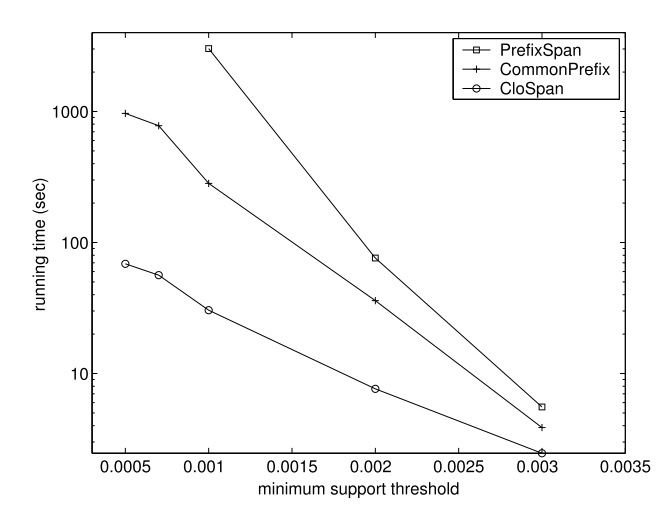
\includegraphics[width=0.8\linewidth]{experiment_time}}
\caption*{Performance}
\center{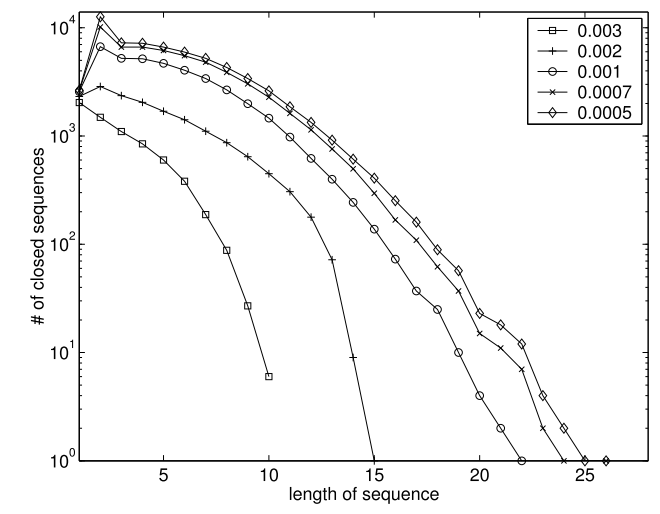
\includegraphics[width=0.8\linewidth]{images/experiment_distribution}}
\caption*{Pattern distribution}
\center{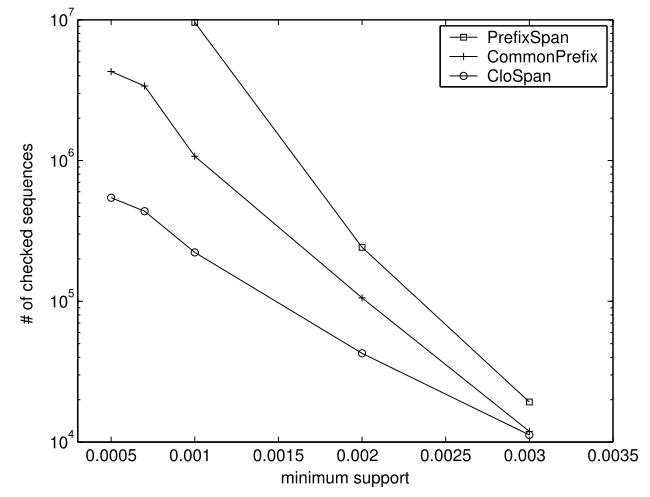
\includegraphics[width=0.8\linewidth]{images/experiment_numchecked}}
\caption*{\# of sequences checked}
\end{figure}

\section{Conclusion}
This approach gives benefits such as:
\begin{itemize}
  \item can mine really long sequences;
  \item produce significantly less number of discovered frequency sequences.
\end{itemize}

More detailed benefits are:
\begin{itemize}
\item Solve closed sequential pattern mining problem;
\item {\it CloSpan} outperforms {\it PrefixSpan} by more than one order of magnitude;
\item capable of mining longer frequent sequences in a large data set with low min\_sup;
\item it does not modify the frequent pattern mining algorithm: it only defines the early termination condition of search branch;
\item this method can be extended to other existing sequential pattern mining algorithms (SPADE, SPAM).
\end{itemize}

\bibliographystyle{unsrt}
\bibliography{references}
\end{document}